\usepackage{pslatex}
\usepackage{listing}
\usepackage{caption}
\usepackage{subcaption}
\usepackage{multirow}

\usepackage{etoolbox}% http://ctan.org/pkg/etoolbox
\AtBeginEnvironment{figure}{\setcounter{subfigure}{0}}% Resets subfigure counter at start of figure environment

\usepackage{tikz}
\usetikzlibrary{shapes,arrows}
\newcommand{\itemv}[1]{\item{#1}}

\tikzset{onslide/.code args={<#1>#2}{%
  \only<#1>{\pgfkeysalso{#2}} % \pgfkeysalso doesn't change the path
}}

\usepackage{scalefnt}

\usetheme[unit=ics]{Frederiksberg}
\useinnertheme{MLHacks}

\AtBeginSection[]
{
	\begin{frame}<beamer>
		\frametitle{Agenda}
		\tableofcontents[currentsection,hideothersubsections]
		\ghostframe
	\end{frame}
}

\title{Local Adaptive Optimization of Time Step}
\subtitle{Experimental plan}
\author{Malte Stær Nissen}
\institute{Datalogisk Institut}
\date{\today}

\begin{document}

\tikzstyle{decision} = [diamond, draw, fill=blue!20, 
    text width=7em, text badly centered, node distance=1.3cm, inner sep=0pt]
\tikzstyle{block} = [rectangle, draw, fill=gray!20, 
    text width=12em, text centered, minimum height=3em]
\tikzstyle{line} = [draw, -latex']
\tikzstyle{cloud} = [draw, ellipse,fill=red!20, node distance=2.3cm, minimum height=2em]

\frame[plain]{\titlepage}

\begin{frame}{Agenda}
	\setbeamercovered{highly dynamic}
	\begin{center}
	\tableofcontents[pausesections,hideothersubsections]
	\end{center}
\end{frame}

\section{The project in short}
\begin{frame}{Short introduction to the project}
    \pause\begin{itemize}[<+->]
		\itemv Materials
        \begin{itemize}
            \itemv In real life: Continuous
            \itemv In simulations: Discrete representations using
                particles/grids
        \end{itemize}
		\itemv Large/detailed materials = huge amount of particles/vertices
        \itemv Varying grid size/scale
        \itemv Simulation of time
        \itemv Reduce avg. number of calculations/time
	\end{itemize}
\end{frame}

\begin{frame}{Illustration of motivation}
    \begin{figure}
        \center
        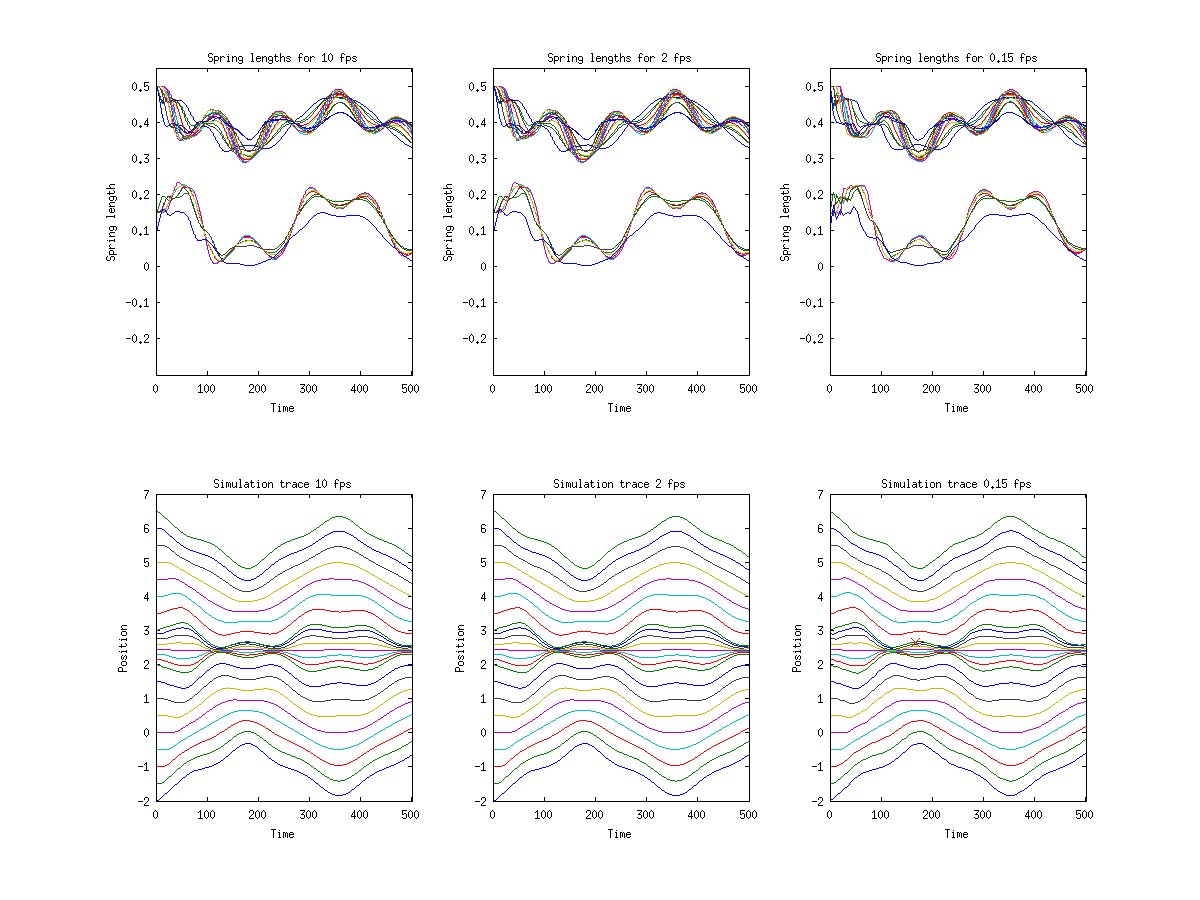
\includegraphics[width=\linewidth,height=6cm]{../images/spring_motivation.png}
        \caption{Simulations of mass spring particle system}
        \label{fig:motivation}
    \end{figure}
\end{frame}

\section{Experimental plan}
\begin{frame}{Overview of experiments}
    \pause\begin{itemize}[<+->]
        \itemv 1D experiments (simple)
        \itemv 2D experiments (more complex)
        \itemv Use experiments to develop schemes
        \itemv Apply methods for uniform meshes 
        \itemv Apply methods for multi-scale meshes
        \itemv Compare method with regular timestepping
    \end{itemize}
\end{frame}

\subsection{1D experiments}
\begin{frame}{1D experiments}
    \pause\begin{itemize}[<+->]
        \itemv 1D for simplicity and ease of development
        \itemv Develop a scheme from experimenting
        \itemv Application: Mass spring particle system (clothes)
        \itemv Hook's law
        \itemv Uniform and multi-scale meshes and simulations
    \end{itemize}
\end{frame}

\subsection{2D experiments}
\begin{frame}{2D experiments}
    \pause\begin{itemize}[<+->]
        \itemv Extend 1D scheme to 2D
        \itemv Gain in complexity
        \itemv Application: Hyperelastic materials
        \itemv Stress and strain
        \itemv Uniform and multi-scale meshes and simulations
    \end{itemize}
\end{frame}

\subsection{Performance experiments}
\begin{frame}{Performance experiments}
    \pause\begin{itemize}[<+->]
        \itemv Total simulation time
        \itemv Compare our 2D scheme with regular time stepping
        \itemv Only sequential tests
        \itemv Only in Matlab
    \end{itemize}
\end{frame}

\end{document}
